\documentclass[11pt]{article}
\PassOptionsToPackage{hyphens}{url}
\usepackage[margin=1in]{geometry}
\usepackage{amsmath,amssymb}
\usepackage{booktabs}
\usepackage{graphicx}
\usepackage{xcolor}
\usepackage{enumitem}
\usepackage{caption}
\usepackage{listings}
\usepackage[numbers,sort&compress]{natbib}
\usepackage[colorlinks=true,linkcolor=blue!50!black,citecolor=blue!50!black,urlcolor=blue!50!black]{hyperref}
\captionsetup{font=small,labelfont=bf}
\setlist{nosep,leftmargin=1.4em}
\emergencystretch=3em

% notation
\newcommand{\sig}{\ensuremath{\sigma}}
\newcommand{\sigp}{\ensuremath{\sigma^{+}}}
\newcommand{\Kfull}{\textsc{full}}
\newcommand{\Kko}{\textsc{knockout}}
\newcommand{\Kdose}{\textsc{dose}}
\newcommand{\phat}{\ensuremath{\hat p}}
\newcommand{\ub}{\ensuremath{\mathrm{UB}_{95}}}
\newcommand{\Katt}{\ensuremath{K_{\mathrm{att}}}}
\newcommand{\Ktrain}{\ensuremath{K_{\mathrm{train}}}}
\newcommand{\Kuni}{\ensuremath{K_{\mathrm{uni}}}}
\newcommand{\Kpub}{\ensuremath{K_{\mathrm{pub}}}}
\newcommand{\Kadapt}{\ensuremath{K_{\mathrm{adapt}}}}
\newcommand{\dcov}{\ensuremath{\Delta_{\mathrm{cov}}}}
\newcommand{\KT}{\ensuremath{\mathcal{D}}}
\newcommand{\KTko}{\ensuremath{\mathcal{D}^{-}}}
\newcommand{\KTdose}{\ensuremath{\mathcal{D}^{1\%}}}
\newcommand{\run}[1]{\textsf{#1}}
% reading copy (librarian, 2026-10-14): marks each change made from the review of run create-or-elicit-paper
\newcommand{\rv}{\textcolor{red!55!black}{\textit{[review]}}}

\lstset{basicstyle=\ttfamily\footnotesize,columns=fullflexible,keepspaces=true,breaklines=true,escapeinside={(*}{*)},
  literate={¬}{{$\neg$}}1 {→}{{$\to$}}1 {∧}{{$\land$}}1 {∨}{{$\lor$}}1 {⊢}{{$\vdash$}}1}

\title{Did Expert Iteration Create It?\\[0.3em]\large A Pretraining Knockout and Compute-Matched Budgets\\in a From-Scratch Theorem Prover}
\author{Dan Pandori et al.\ (author list for Dan to decide)}
\date{Draft of 2026-10-13; reading copy with the review's corrections, 2026-10-14. Not for circulation.}

\begin{document}
\maketitle

\begin{center}\fbox{\parbox{0.94\linewidth}{\small\textbf{Reading copy (librarian, 2026-10-14).} This is the draft written by run \run{create-or-elicit-paper} (fork \texttt{dan-pandori/nd-takehome}, branch \texttt{dan\_create-or-elicit-paper}, commit \texttt{ed8cf1ea}), with the corrections from its review (\texttt{review\_create-or-elicit-paper.md}, commit \texttt{1ad2a691}) applied. Each change is marked \rv{}. No headline number changed. The review found no hard-constraint violation, and nothing was quarantined.}}\end{center}

\begin{abstract}
Reinforcement learning against a verifier improves reasoning models. Whether it creates capabilities the base lacked
or raises the probability of behaviour the base already had is contested, and large-model studies can rarely change
what the base saw. We study the question in a 9.56M-parameter transformer prover, trained from scratch on 155,000
synthetic natural-deduction proofs of propositional logic, judged only by Lean~4, with exact likelihoods for any
proof. We remove one inference composition from pretraining, the classical reductio \sig{} (double-negation
elimination applied to a refuted negation), refill the data to the same size, and run 16 rounds of expert iteration.
In a pre-registered test, no \sig-free base acquired a classical theorem family (0/6 seeds), against 6/6
full-exposure seeds (one-sided Boschloo $p=0.00024$). Counting only families acquired during RL: 5/6 vs 0/6
($p=0.0032$). Restoring \sig{} in 1\% of pretraining restored acquisition on 3/3 seeds. The knockout bases were not
\sig-free: four of six wrote \sig{} proofs of held-out family members (1--6 in 1.1--1.4 million attempts), only two
are certified out of reach at RL's compute budget, and the one knockout run that made progress did so mostly on
members its base could already reach. Measurement matters too: of the 51--60 theorems per seed that RL
``creates'' at equal sample counts, 14--21 remain once the base gets RL's compute as attempts, under every budget
allocation tried. In this organism, expert iteration amplified a composition pretraining had exposed, even at 1\%,
but did not build it within 16 rounds from a base that had never seen it.

\end{abstract}

\section{Introduction}
\label{sec:intro}

Reinforcement learning against a verifier is now the standard way to improve reasoning models. Whether it teaches them
anything new is contested. \citet{yue2025doesrl} find that base models overtake their RL-trained descendants in
pass@$k$ as $k$ grows. \citet{karan2025power} approach RL's gain on a mathematics benchmark by sampling the base from a
sharpened distribution, with no training. Other work reports RL solving problems the base never solved
\citep{abdulsalam2026rewrite,liu2025prorl}. Part of the disagreement is about budgets. A base whose per-attempt
success probability on a problem is $10^{-6}$ will almost never solve it in 1,024 attempts, yet the capability is
present in a sense that matters for evaluation and safety. A capability is defined only relative to a sampling budget
\citep{li2026elicitcreate,brown2024monkeys}.

A claim that RL \emph{created} a capability therefore needs three things:
\begin{itemize}
\item a budget at which the base is judged unable, tied to what RL spent;
\item controls that receive RL's training without RL's proofs;
\item ideally, a base that never had the capability \citep{jain2023mechanistically,deeb2024unlearning}.
\end{itemize}
Pretraining interventions before RL exist. \citet{zhang2025interplay} vary a context's share of pretraining (0\%,
0.1\%, 1\%) in a 100M model and find no RL transfer below 1\%. \citet{abdulsalam2026rewrite} exclude shortcuts from
pretraining and see GRPO build them. \citet{tsilivis2025rlntp} set the share of long demonstrations exactly. We add a
narrower intervention, with the base's own rate measured. We remove a single inference composition from pretraining,
keep both of its parts, refill the data to the same size, and measure the base's rate for the composition at about a
million attempts.

We do this in a model organism small enough to allow it. It is a 9.56M-parameter transformer prover for propositional
logic, pretrained from scratch on 155,000 synthetic natural-deduction proofs. It acts through a proof-state interface,
one inference step at a time, and Lean~4 alone decides whether a proof counts. The composition we remove is the
classical reductio \sig{}: to prove a positive goal $G$, assume $\neg G$, derive a contradiction, conclude $\neg\neg G$
by negation introduction, and eliminate the double negation (\texttt{DN}, Lean's \texttt{Classical.byContradiction}).
Both rules stay in the data, used separately. We track six classical theorem families, such as excluded middle and
Peirce's law, whose \emph{strict} members can only be proved by eliminating a double negation the proof itself built.
Their 106 held-out strict theorems are never trained on. We then run expert iteration (EI) from each base: sample,
keep what Lean accepts, fine-tune, for 16 rounds (Fig.~\ref{fig:overview}).

\begin{figure}[t]
\centering
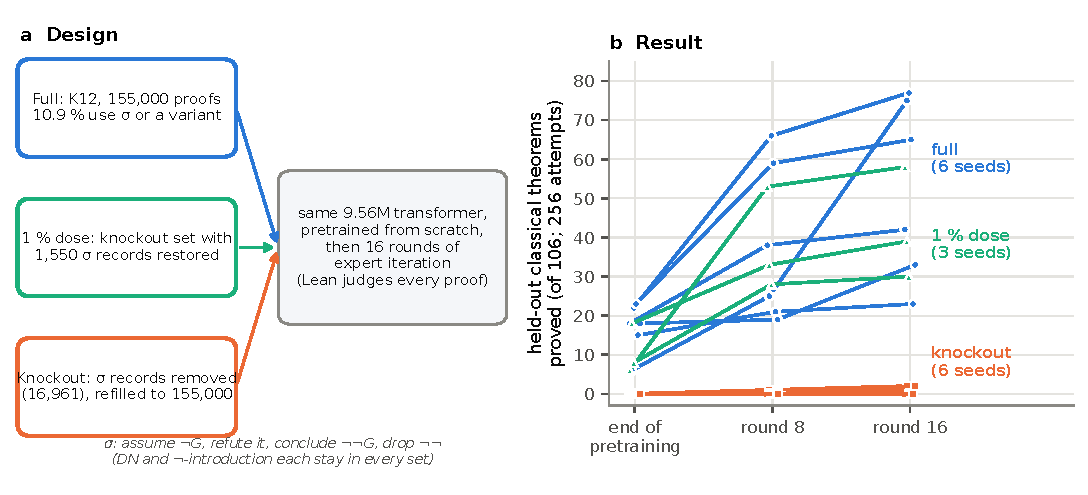
\includegraphics[width=\linewidth]{figures/fig0_overview.pdf}
\caption{\textbf{Design and result.} (a) Three pretraining sets that differ only in the classical reductio \sig{}. (b)
Held-out classical theorems proved (of 106, with 256 attempts each) at the end of pretraining and after 8 and 16 rounds
of expert iteration, one line per seed. No knockout seed acquires a classical family in 16 rounds.}
\label{fig:overview}
\end{figure}

\paragraph{Two objections, and the null model.} The first objection is that a model cannot learn what it never saw.
But the knockout bases saw both rules, and they still write \sig{}: five of six proved held-out strict theorems with it
at large sample sizes. The second objection is stronger. At the bases' measured rates, EI's 3,936 attempts per round on
the 123 strict training theorems should find at most 0.02 \sig{} proofs per round. A first success would then be
expected only after 47 rounds or more. We take this
waiting-time arithmetic as the null model and ask what happens beyond it.

\paragraph{Results.}
\begin{itemize}
\item \textbf{No knockout seed acquired a classical family in 16 rounds} (0/6, which bounds the per-seed rate below
0.39), against 6/6 full-exposure seeds. That pre-registered contrast is largely decided before RL: one family is
already acquired at the end of pretraining on 5/6 full seeds. The contrasts specific to RL were not pre-registered.
During RL, full seeds gained 8--69 held-out strict theorems and knockout seeds 0--2 (exact Mann--Whitney $p=0.0011$).
Five of six full seeds against none acquired a family during RL ($p=0.0032$; on the three seeds that shared the
knockout's hardware, 2/3 vs 0/6, $p=0.034$).
\item \textbf{One percent is enough.} Restoring \sig{} in 1\% of pretraining records restored acquisition on 3/3 seeds.
\item \textbf{Beyond the null.} The knockout ladders wrote \sig{} from round 1 on theorems that supply the double
negation, and trained on 844--4,428 such proofs. Three of six reached a strict training theorem sooner than their bases'
rates predict: 0.55 seeds expected by round 16, 3 observed, $p=0.006$ under the null. None carried the step to a
family. The ladder that went furthest, continued to 24 rounds, proved 5 of the 106 held-out theorems, more often each
round, and no more of them.
\item \textbf{Measurement.} In three earlier full-exposure runs, 51--60 theorems per run look RL-created at equal
sample counts. Only 14--21 remain when the base gets RL's compute as attempts, under every budget allocation we tried.
\end{itemize}

\paragraph{Contributions.}
\begin{enumerate}
\item \textbf{A composition knockout in pretraining} (\S\ref{sec:results}), with a dose arm and diagnostics that
separate ``absent'' from ``rare'': base rates at about $10^6$ attempts, certificates, a waiting-time null, and
likelihoods of known proofs along every RL run. It was pre-registered, with six seeds per main arm, and an analyst who
did not write the experiment's code recounted it independently.
\item \textbf{A compute-matched measurement protocol, applied end to end} (\S\ref{sec:setup}, \S\ref{sec:case}). It
gives the base a budget of attempts matched to RL's compute under several defensible allocations, so that the
``created'' set becomes a curve in the budget. It brackets each theorem's success rate between sampling bounds and a
likelihood estimate, certifies unreachability, and nets out RL-free training. It integrates budget-relative definitions
from prior work \citep{li2026elicitcreate,davidson2023retraining,wu2025invisibleleash}.
\item \textbf{An open organism}: a from-scratch prover with a sound judge, likelihoods of arbitrary proofs at every
checkpoint, and pretraining that can be edited one composition at a time. Code, data, checkpoints and per-arm compute
are public.
\end{enumerate}

\paragraph{What transfers.} The protocol and the waiting-time logic transfer to larger models; the numbers do not. The
1\% threshold, the $10^{-6}$ rates and the dynamics of EI belong to this organism, and they depend on how many training
problems need the composition. Two lessons follow, with that caveat. Failure at modest $k$ does not show absence: our
knockout bases fail at $k=256$, yet succeed at pooled rates near $10^{-6}$ per attempt, and at up to about
$5\times10^{-4}$ on a few theorems. And removing a
composition from pretraining kept this RL from acquiring it within 16 rounds, but 1\% of the data restored it.
Section~\ref{sec:discussion} discusses what other algorithms and injected demonstrations did to similar patterns in
earlier, smaller organisms.

\section{The organism}
\label{sec:setup}

\paragraph{Logic, data and judge.} Theorems are sequents of propositional logic over four atoms
($\Gamma \vdash G$, with $\land,\lor,\to,\neg,\bot$). Proofs are Fitch-style natural deduction: premises,
assumptions that open boxes, and the introduction and elimination rules for each connective, plus $\bot$-elimination
and double-negation elimination (\texttt{DN}). The pretraining set \KT{} holds 155,000 synthetic proofs of 2--12 lines
from a generator, with a flat length distribution. Every rule the RL models use occurs in at least 8.0\% of its
records. A proof counts if and only if Lean~4 core accepts its rendering as a Lean proof term. A syntactic pre-filter
may reject malformed text before Lean sees it, but it never accepts anything on its own. The pre-filter's false-reject
rate on a re-checked sample is 0 of 1,950 (\S\ref{sec:robust}). An older in-house checker is not used for any number
here.

\paragraph{Model and interface.} Every model is the same network: a decoder-only transformer with 6 layers of width
384 and ALiBi and NoPE attention heads, with 9,560,832 parameters. It is pretrained from scratch for 1,200\,s on one
NVIDIA A40 (about 24,000 steps, Muon and AdamW, with an auxiliary multi-token-prediction loss). That is about 3.7
passes over the (state, action) pairs of \KT{}. The model acts in a \emph{proof-state environment}. It sees the
focused goal's Lean tactic state (hypotheses in scope and the goal) and writes one step, such as
\texttt{have n5 : $\neg$P := n1 n4}. The environment applies the step, assigns the line names, opens and closes the
boxes for $\to$- and $\neg$-introduction and the branches of $\lor$-elimination, and stops the attempt at the first
step it cannot apply. The finished proof is rendered in Lean and judged. Figure~\ref{fig:lean} shows two proofs written by
a model in this paper.

\paragraph{Expert iteration.} RL is ``T1'' expert iteration \citep{anthony2017exit}, the variant with uniform
allocation. In each round the current model samples $k=32$ attempts at temperature $T=0.8$ for each of 4,495 training
theorems (\texttt{rl\_targets}). Lean checks every attempt. Accepted proofs accumulate across rounds, up to four per
theorem. The model is then fine-tuned for 600 steps on those proofs (each weighted four times) mixed with 20,000
records replayed from its own pretraining set. We run 16 rounds. Every round also samples $k=32$ attempts on 832
tracked held-out theorems, which are never trained on. We write \emph{pend} for the end of pretraining and
\emph{r$N$} for the model after $N$ rounds.

\paragraph{Reads.} A \emph{plain read} draws $k=256$ independent attempts per theorem at $T=0.8$, with at most 96 steps
and 512 tokens per step. A theorem is \emph{solved} if at least one attempt is accepted. Two sample seeds give two draws
(x0, x1) of the same checkpoint. A \emph{guided read} uses the same budget, but a step rejected by a per-step logical
checker is redrawn from the same state without replacement, up to 10 times per attempt. The checker never rejected a
step Lean accepts in 314,541 tested (state, step) pairs (run \run{guided-tts}; run names refer to the reviewed reports listed
in Appendix~\ref{app:provenance}). Evaluation theorems are never trained on.
They are textbook72 (72 textbook problems, used only for scoring); holdout250 (250 generator theorems); together these
are ``the 322''. The other sets are the held-out members of the theorem families below and \texttt{p2/heldout} (5,000
generator theorems read greedily, for general ability).

\begin{figure}[t]
\centering
\begin{minipage}{0.96\linewidth}
\small
\emph{(a)} $\neg S \to \neg P,\ P \vdash R \to S$ (\texttt{la\_transfer\_916}), one of knockout seed 1's base's rare
large-$k$ successes. Assume $R$; assume $\neg S$ and refute it, which gives $\neg\neg S$ by $\neg$-introduction; then
\texttt{DN}:
\begin{lstlisting}
theorem t (P Q R S : Prop) (h1 : ((¬S) → (¬P))) (h2 : P) : (R → S) := by
  have n1 : ((¬S) → (¬P)) := h1
  have n2 : P := h2
  have n9 : (R → S) := (fun (n3 : R) => by
    have n7 : (¬(¬S)) := (fun (n4 : (¬S)) => by
      have n5 : (¬P) := n1 n4
      have n6 : False := n5 n2
      exact (n6 : False))
    have n8 : S := Classical.byContradiction (fun hh => n7 hh)
    exact n8)
  exact n9
\end{lstlisting}
\emph{(b)} The same base on a held-out member of the converse-contraposition family,
$\neg S \to \neg((S\land R)\lor R) \vdash ((S \land R) \lor R) \to S$ (\texttt{la\_transfer\_1246}): the same \sig{}
step, then \texttt{DN} in both branches of an $\lor$-elimination.
\end{minipage}
\caption{\textbf{The classical reductio \sig{} in Lean, written by a knockout base before any RL.} Both proofs are
accepted by Lean and rejected when the goal is negated (\texttt{paper/scripts/lean\_examples.py}). No record of the
knockout pretraining set \KTko{} contains a \texttt{DN} step on a derived double negation.}
\label{fig:lean}
\end{figure}

\paragraph{The composition \sig{} and the theorem families.} \sig{} is a \texttt{DN} step whose cited line was built
by $\neg$-introduction: Lean's \texttt{Classical.byContradiction} applied to a refutation of $\neg G$ that the proof
itself constructed. \sigp{} widens this to a \texttt{DN} step that cites any derived line. The \emph{lemma route}
proves $\neg\neg G \to G$ inside an implication box and applies it, and so avoids \texttt{DN} on a derived line. In
\KT{}, \sig{} occurs in 16,703 records and \sigp{} in 16,961 (10.94\%). The lemma route occurs in none. We track six
classical generator families: converse contraposition ($\neg B \to \neg A \vdash A \to B$), negated conditional
($\neg(A\to B) \vdash A \land \neg B$), Peirce's law, the Peirce sequent ($(A\to B)\to A \vdash A$), excluded middle,
and De Morgan $\neg(A\land B) \vdash \neg A \lor \neg B$. Each member is a substitution instance. Each family has 40
trained members (in \texttt{rl\_targets}) and 40 held-out members (sampled every round, never trained on). A member is
\emph{classical-only} if a complete intuitionistic decision procedure (G4ip) finds no proof. It is \emph{strict} if it
is classical-only and no subformula of its sequent is a double negation. Any proof of a strict member must then apply
\texttt{DN} to a double negation the proof built itself: by \sig{}, another \sigp{} route, or the lemma route. There are
123 strict trained members and 106 strict held-out members (Table~\ref{tab:families}). The latter are 105 family
members plus one generated theorem, \texttt{la\_transfer\_916} (Fig.~\ref{fig:lean}a).

\begin{table}[t]
\centering\small
\caption{Strict members per family (classical-only, no $\neg\neg$ subformula in the sequent). Every proof of a strict
member must eliminate a double negation the proof itself builds. The held-out total adds one generated theorem.}
\label{tab:families}
\setlength{\tabcolsep}{4pt}
\begin{tabular}{lcccccc|c}
\toprule
 & contrap.\ conv. & neg.\ cond. & Peirce & Peirce seq. & excl.\ middle & De Morgan & total \\
\midrule
trained (of 40 each) & 27 & 16 & 15 & 18 & 38 & 9 & 123 \\
held-out (of 40 each) & 18 & 15 & 12 & 19 & 37 & 4 & 105 + 1 \\
\bottomrule
\end{tabular}
\end{table}

\paragraph{Arms.} All arms share the network, the pretraining recipe and the EI protocol. Only the pretraining data
differs (Table~\ref{tab:arms}).
\begin{itemize}
  \item \Kfull{} pretrains on \KT{}. Seeds s0--s2 come from earlier runs: rounds 1--8 ran on RTX A6000 cards at
  sampling batch 2,048 (s2 at 1,024 from round 2), and rounds 9--16 on A40s. Seeds s3--s5 are new, with every round
  on A40s at batch 1,024.
  \item \Kko{} pretrains on \KTko{}. It is \KT{} minus exactly the 16,961 \sigp{} records, refilled with 16,961 records
  drawn per length from \KT{}'s own unused source pools. Every refill record passes every \KT{} filter and contains no
  \sigp{} or lemma route. Under both renaming-invariant keys, the refill shares no theorem class with \KT{} or with any
  evaluation file. Per-length counts are identical to \KT{}'s, and Lean accepts all 16,961 refill records.
  \texttt{DN} and $\neg$-introduction each remain (\texttt{DN} on premises and assumptions in 3.29\% of records);
  only their composition is gone.
  \item \Kdose{} pretrains on \KTdose{}: \KTko{} with 1,550 refill records swapped back for removed \sig{} records,
  at \KT{}'s length mix. The \sigp{} share is exactly 1.00\%.
\end{itemize}
Arms with the same seed number share initial weights and per-round sampling seeds, not data. A change of sampling
batch only re-draws samples, because Lean checks every sample. Old and new full seeds are pooled in every comparison
below.

\begin{table}[t]
\centering\small
\caption{Arms. Every model: 9,560,832-parameter transformer, proof-state interface, trained from scratch (1,200\,s),
then T1 expert iteration (16 rounds; $k=32$, $T=0.8$, 600 fine-tune steps per round, 4,495 training theorems). Lean~4
alone judges.}
\label{tab:arms}
\begin{tabular}{llcl}
\toprule
arm & pretraining set & seeds & \sigp{} share of records \\
\midrule
\Kfull{} & \KT{} (155,000 records) & 6 (s0--s5) & 10.94\% \\
\Kko{} & \KTko{}: \KT{} $-$ 16,961 \sigp{} records $+$ 16,961 refill & 6 (s0--s5) & 0 \\
\Kdose{} & \KTdose{}: \KTko{} with 1,550 \sig{} records restored & 3 (s0--s2) & 1.00\% \\
\bottomrule
\end{tabular}
\end{table}

\section{Results: the \sig{} knockout}
\label{sec:results}

All numbers in this section are on the 9.56M-parameter models of Table~\ref{tab:arms}, judged by Lean alone, from the
evaluation with sample seed x0 unless stated. An analyst who had not written the experiment's code recounted every count
in this section from the raw files, with separate code, and re-checked the proofs in Lean. Numbers computed for this
paper are marked (\emph{this paper}); they are recomputed from those recounted files.

\subsection{No knockout seed acquired a family in 16 rounds}
\label{sec:primary}

\begin{table}[t]
\centering\small
\caption{Strict held-out theorems proved (of 106) per seed at r0 (end of pretraining), r8 and r16, and the families
acquired. x0 and x1 are two sample seeds; ``guided'' is the guided evaluation. Families: cc = converse contraposition,
nc = negated conditional, pe = Peirce, ps = Peirce sequent, em = excluded middle; families acquired already at r0 are
underlined. $\dagger$ = seeds from earlier runs (other GPU class and batch in rounds 1--8). The dose arm's other
evaluations are in Appendix~\ref{sec:checks}.}
\label{tab:primary}
\begin{tabular}{lrrrrrll}
\toprule
model & r0 & r8 & r16 x0 & r16 x1 & guided & acquired at r16 (x0) & gain r0$\to$r16 \\
\midrule
\Kfull{} s0$^\dagger$ & 18 & 38 & 42 & 43 & 44 & \underline{cc}, nc & 24 \\
\Kfull{} s1$^\dagger$ & 6 & 25 & 75 & 73 & 75 & cc, em, pe & 69 \\
\Kfull{} s2$^\dagger$ & 22 & 66 & 77 & 77 & 80 & \underline{cc}, nc, pe, ps & 55 \\
\Kfull{} s3 & 23 & 59 & 65 & 64 & 64 & \underline{cc}, nc, pe, ps & 42 \\
\Kfull{} s4 & 15 & 21 & 23 & 22 & 24 & \underline{cc} & 8 \\
\Kfull{} s5 & 18 & 19 & 33 & 34 & 33 & \underline{cc}, ps & 15 \\
\midrule
\Kko{} s0 & 0 & 0 & 0 & 0 & 0 & -- & 0 \\
\Kko{} s1 & 0 & 1 & 2 & 2 & 3 & -- (r20: 5; r24: 5) & 2 \\
\Kko{} s2 & 0 & 0 & 1 & 1 & 0 & -- & 1 \\
\Kko{} s3 & 0 & 0 & 0 & 0 & 0 & -- & 0 \\
\Kko{} s4 & 0 & 0 & 0 & 0 & 0 & -- & 0 \\
\Kko{} s5 & 0 & 0 & 2 & 1 & 2 & -- & 2 \\
\midrule
\Kdose{} s0 & 6 & 53 & 58 & & & cc, nc, pe, ps & 52 \\
\Kdose{} s1 & 18 & 33 & 39 & & & \underline{cc}, nc & 21 \\
\Kdose{} s2 & 8 & 28 & 30 & & & cc, nc & 22 \\
\bottomrule
\end{tabular}
\end{table}

No knockout seed acquired any classical family by r16; every full seed had at least one (Table~\ref{tab:primary},
Fig.~\ref{fig:endpoint}). This is the pre-registered primary indicator, 6/6 against 0/6, one-sided Boschloo
$p = 0.00024$. The same holds in the second sample seed, in the guided evaluation, and with the looser held-out sets
first pre-registered (178 theorems; they were replaced by the strict sets in a dated amendment after round 1 of the
first knockout ladder, because that base proved 136 of 155 generated ``classical'' targets using a $\neg\neg$ the
sequent supplied). The 0/6 bounds the per-seed rate at which this EI acquires a family from a \sig-free base below 0.39
(one-sided 95\%).

The indicator is a weak statement about RL, however. Converse contraposition is acquired \emph{before} RL on 5/6 full
bases (6/6 in the guided evaluation). Applied to the bases, the indicator already gives 5/6 against 0/6 ($p = 0.0032$),
or 6/6 against 0/6 in the guided evaluation ($p = 0.00024$). Per family, the pre-registered rule gives
\textsc{needs exposure} only for converse contraposition (6 vs 0 seeds; Holm-corrected over six families, 0.0015). It
gives \textsc{undetermined} for negated conditional, Peirce and the Peirce sequent (3 vs 0 each; $p = 0.034$, Holm 0.17)
and for excluded middle (1 vs 0), and \textsc{neither} for De Morgan, whose four strict members no model proves.

The comparisons specific to RL were not pre-registered. During RL, the full seeds gained 24, 69, 55, 42, 8 and 15 strict
held-out theorems and the knockout seeds 0, 2, 1, 0, 0 and 2: the arms do not overlap (exact one-sided Mann--Whitney
$U = 36$, $p = 0.0011$). Counting only families acquired between r0 and r16, it is 5/6 against 0/6 ($p = 0.0032$). The
old full seeds ran rounds 1--8 on other hardware. Restricted to the three new full seeds, it is 2/3 against 0/6
($p = 0.034$). On the training side, the knockout ladders proved none of the 123 strict training theorems in round 1
and only 0, 5, 1, 0, 0 and 2 of them by round 16. The full ladders went from 21, 1, 27, 17, 15 and 20 in round 1 to 49,
80, 86, 78, 33 and 36 (Fig.~\ref{fig:dynamics}a). No knockout ladder ever had proofs for half of any family's strict
training theorems.

\begin{figure}[t]
\centering
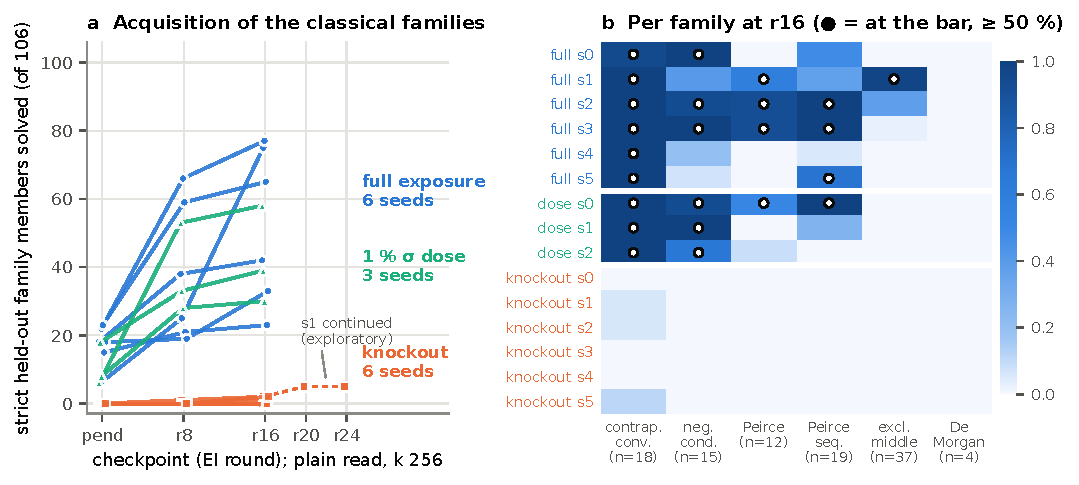
\includegraphics[width=\linewidth]{figures/fig1_endpoint.pdf}
\caption{\textbf{Per seed and per family.} (a) Strict held-out theorems proved at r0, r8 and r16; knockout seed 1 was
continued to r24 (dashed; exploratory). (b) Share of each family's strict held-out members proved at r16; a dot marks
an acquired family ($\geq 50\%$).}
\label{fig:endpoint}
\end{figure}

\subsection{One percent is enough}
\label{sec:dose}

The dose bases proved 6, 18 and 8 strict held-out theorems at r0, and 58, 39 and 30 at r16. All three acquired families
during RL; dose s1 had already acquired converse contraposition at r0. That is 3/3 against the knockout's 0/6
(Boschloo $p = 0.0033$; this arm was added by a dated amendment before it ran, and is exploratory). At r16 the dose seeds
lie inside the full arm's range (two-sided Mann--Whitney $p = 0.55$ with three seeds; \emph{this paper}). In round 1 the
dose bases wrote 223, 183 and 241 \sig{} proofs, and the free positive reductio from round 1 on. The new full seeds
wrote 635--885 \sig{} proofs and the knockout seeds 6--13. The dose changes the data around \sig{} far less than the
knockout removed. In \KTdose{}, \texttt{DN} appears in 4.24\% of records and $\neg$-introduction in 6.12\%, against 3.29\% and 5.19\% in \KTko{} and 13.73\% and 15.21\% in \KT{}. Classical-only theorems are 1.56\% of a 20,000-record sample, against 1.35\% and 4.17\% (\emph{this paper}, from the dose set's file). A second sample seed and a guided evaluation of the dose arm, run for this paper, agree. The second seed
proves 56, 39 and 30 strict theorems, and the guided evaluation proves 58 and 42 on seeds 0 and 1 (seed 2 pending). All three seeds acquire the same families
as in the first evaluation (Appendix~\ref{sec:checks}).

\subsection{\sig{} is rare in the knockout arm, not absent}
\label{sec:rare}

\paragraph{The bases, sampled about a million times.} We drew 1.1--1.5 million attempts from each knockout base, spread
over the 106 strict held-out theorems (about $10^4$ per theorem, with sampling on a theorem paused after its first
success in each block of 1,024). Five of the six bases proved strict theorems: seed 1 seven times, seed 4 three times,
seed 5 twice, and seeds 2 and 3 once each. Every success is a genuine \sig{} proof, and twelve of the fourteen are on
family members, eleven of them converse contraposition. Seed 3's single success is on the generated theorem
\texttt{la\_transfer\_916}. Pooled rates are 0 to $6\times10^{-6}$ per attempt; on the theorems with a success, the
per-theorem estimates are $7.5\times10^{-5}$ to $4.9\times10^{-4}$, each from one to three successes.

\paragraph{Certificates.} As pre-registered, pooled over the 106 theorems at each seed's $\Ktrain(16)$, only seed 0's
base is certified out of reach: 0 successes in 1.50 million attempts, $\mathrm{UB}_{95} = 1.99\times10^{-6} <
0.05/K = 2.14\times10^{-6}$ (Table~\ref{tab:certs}). Its certificate holds up to $K = 25{,}112$, 8\% above the budget,
and only at this one allocation and $N_{\mathrm{eval}}$. Pooled over the 105 family members alone, as the experiment
reported it, seed 3 is also certified; the difference is its success on \texttt{la\_transfer\_916}. No family is
certified for any seed: at this sampling the largest certifiable $K$ per family is 717--8,772. A pooled certificate
bounds the mean rate over the pool, not any theorem in it.

\begin{table}[t]
\centering\small
\caption{Knockout bases at large $k$, pooled over the 106 strict held-out theorems (the pre-registered pool), at each
seed's $K = \Ktrain(16)$. Certified out of reach if $\mathrm{UB}_{95} < 0.05/K$; $K_{\max} = 0.05/\mathrm{UB}_{95}$ is
the largest budget the data certify. In parentheses: the 105 family members only (excluding
\texttt{la\_transfer\_916}).}
\label{tab:certs}
\begin{tabular}{lrrrrc}
\toprule
knockout base & $K$ & attempts & successes & $K_{\max}$ & certified \\
\midrule
s0 & 23,322 & 1,504,600 & 0 (0) & 25,112 (24,892) & yes (yes) \\
s1 & 17,189 & 1,122,426 & 7 (6) & 4,268 (4,730) & no (no) \\
s2 & 20,907 & 1,350,143 & 1 (1) & 14,230 (14,106) & no (no) \\
s3 & 20,782 & 1,342,688 & 1 (0) & 14,152 (22,376) & no (yes) \\
s4 & 21,554 & 1,372,403 & 3 (3) & 8,850 (8,772) & no (no) \\
s5 & 22,297 & 1,432,256 & 2 (2) & 11,375 (11,275) & no (no) \\
\bottomrule
\end{tabular}
\end{table}

\paragraph{The ladders.} Every knockout ladder wrote \sig{} in round 1, 6--13 distinct proofs per ladder, on theorems
that supply $\neg\neg G$ or whose goal is a negation. Over their rounds, the fine-tuning mixes carried 844--4,428 such
self-written \sig{} records (2,948--9,140 \sigp{}). The free positive reductio was another matter. Over 16 rounds the
knockout ladders produced 0, 34, 4, 1, 2 and 16 distinct proofs using it, first in rounds never, 9, 12, 15, 15 and 2.
The full ladders produced 17,507--50,222 each, and the dose ladders 20,597--26,662, from round 1
(Fig.~\ref{fig:dynamics}b). EI thus trained on \sig{} in easy contexts from the start and did not carry the step to
the theorems that need it.

\begin{figure}[t]
\centering
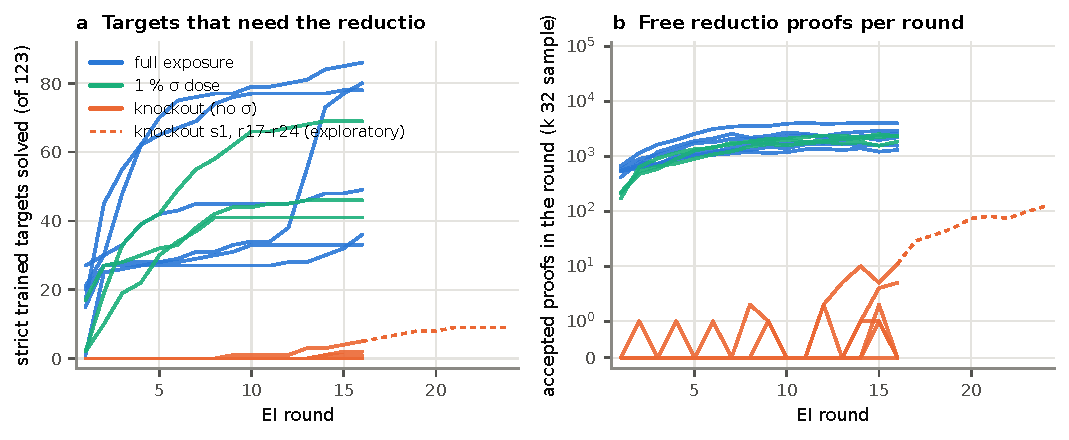
\includegraphics[width=\linewidth]{figures/fig2_dynamics.pdf}
\caption{\textbf{Ladder dynamics.} (a) Strict training theorems (of 123) with an accepted proof so far. (b) Accepted
proofs per round, in each round's $k=32$ sample over all 4,495 training theorems, that use a free positive reductio
(symmetric-log scale). Full and dose ladders write hundreds from round 1 and thousands later. Four knockout ladders
write a few, late. Knockout s1 (dashed beyond round 16) spreads it, from 11 in round 16 to 123 in round 24.}
\label{fig:dynamics}
\end{figure}

\paragraph{Beyond the waiting-time null (\emph{this paper}, post hoc).} Suppose each knockout ladder kept sampling the
123 strict training theorems at its base's pooled rate. It would then expect a first strict success after 47 (seed 1),
115 (seed 4), 180 (seed 5) and 340 (seed 2) rounds, and never for seeds 0 and 3. The expected number of seeds with a
strict success by round 16 is 0.55. Three had one: seed 1 in round 9, seeds 2 and 5 in round 14. Under the null that is
a $p = 0.006$ event. So EI did raise the knockout models' rate of the free positive reductio, presumably through the
\sig{} it practised on easier theorems, but not by enough to acquire a family. The two certified-on-105 bases (s0, s3)
never produced one.

\paragraph{Likelihood.} We scored the best known \sig{} proof of each of 101 strict held-out theorems under every
checkpoint, teacher-forced at $T=0.8$ (Fig.~\ref{fig:logp}). The proofs are the full ladders' own. At r0 the median
log-probability is $-15.4$ to $-20.9$ nats under the four full bases scored, $-18.9$ to $-25.3$ under the dose bases,
and $-26.0$ to $-36.0$ under the knockout bases. The arms overlap only between dose and knockout seed 1. The step that
costs most is the box that assumes $\neg G$: $-18.0$ to $-21.6$ nats under the knockout bases, $-10.5$ under full seed
0's base. From r0 to r16, two ladders move strongly toward these proofs (full s3 $+10.3$ nats, dose s0 $+16.6$). The
other full and dose ladders move $+1.7$ to $+4.3$, and the knockout ladders $-7.6$ to $+3.7$. Several knockout ladders
rise by 5--8.5 nats by r4 and fall back. Two caveats apply. The scores use one of the 33 line-numbering offsets, so
they understate a proof's probability by at most $\ln 33 \approx 3.5$ nats. And a knockout ladder that found its own
spelling (seed 1, below) need not raise these.

\begin{figure}[t]
\centering
\begin{minipage}{0.49\linewidth}
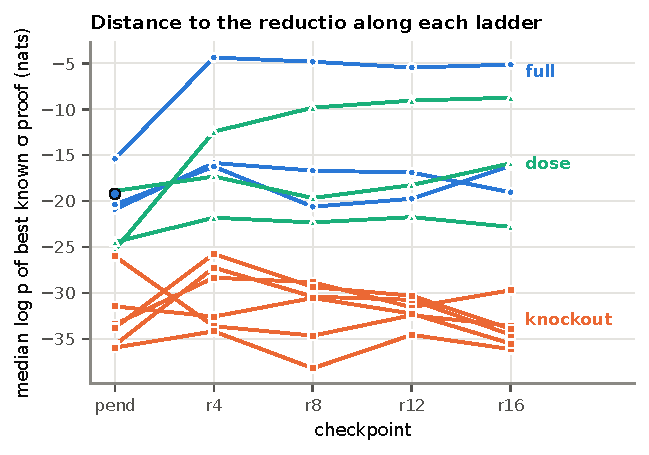
\includegraphics[width=\linewidth]{figures/fig3_logp.pdf}
\caption{Median log-probability of the best known \sig{} proof of the strict held-out theorems, along each ladder (one
line-numbering offset, $T=0.8$). The outlined point is full seed 0's base, whose ladder was not rescored.}
\label{fig:logp}
\end{minipage}\hfill
\begin{minipage}{0.49\linewidth}
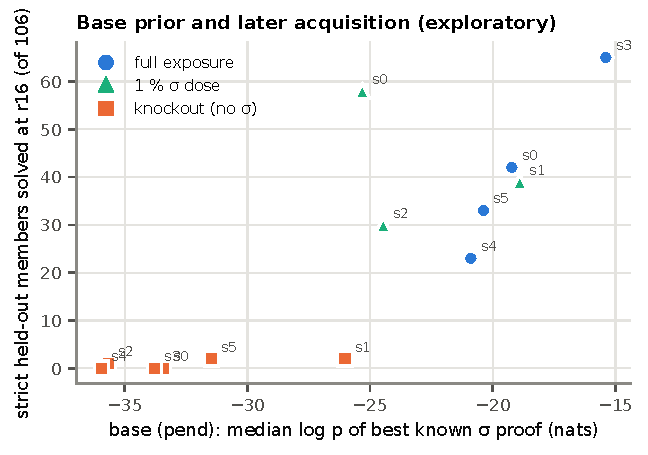
\includegraphics[width=\linewidth]{figures/fig6_prior.pdf}
\caption{Exploratory (\emph{this paper}): the base's median log-probability of known \sig{} proofs against strict
held-out theorems proved at r16, for the 13 ladders with a scored base.}
\label{fig:prior}
\end{minipage}
\end{figure}

\subsection{The one knockout ladder that moved}
\label{sec:ko-s1}

Knockout seed 1's free reductio kept spreading, so it was continued to round 24 (exploratory). Its free positive
reductio proofs per round rose from 11 in round 16 to 123 in round 24. From round 21 it had proofs for 9 of the 27
strict converse-contraposition training theorems, and it never went past 9 strict training theorems in all. It proved
the same five strict held-out theorems at r20 and r24, each more often: four converse-contraposition members and
\texttt{la\_transfer\_916}. The largest gain is on \texttt{la\_transfer\_1019}, from 0 to 32 to 214 successes in 256
attempts at r16, r20 and r24. No family was acquired. Its r20 proofs of these theorems take three routes: \sig{} (32
proofs), other \sigp{} (24) and the lemma route (7), a route absent from every pretraining set.

Was this elicitation of something the base already did? In the large-$k$ sample, the base proved four of its 18
converse-contraposition members, each one to three times in 7,168--10,240 attempts. That is within reach by the rate
definition, but every one is below $K$ attempts. Three of the four members the ladder proves (\texttt{1246},
\texttt{1460}, \texttt{2256}) are among them. The fourth, \texttt{1019}, had no base success in about $10^4$ attempts.
A re-sample of these members at $n \geq K$ without early stopping, run for this paper, is pending.

\subsection{What else the knockout changes}
\label{sec:side}

\paragraph{Data.} Removing \sigp{} records also thins its constituents. In \KTko{}, \texttt{DN} appears in 3.29\% of
records (13.73\% in \KT{}) and $\neg$-introduction in 5.19\% (15.21\%). Theorems with no intuitionistic proof fall from
4.17\% to 1.35\% of a 20,000-record sample; the rest use \texttt{DN} on a $\neg\neg$ that a premise or an assumption
supplies. Mean proof term size moves from 35.91 to 36.25 nodes. The knockout removes the composition's co-occurrence,
and also makes each constituent three to four times rarer.

\paragraph{General ability.} The knockout bases are 6.88 points worse at greedy decoding of 5,000 held-out generator
theorems (0.8829 vs 0.9517). The gap comes from the 679 theorems whose reference proof uses \sig{} (0.45 vs 0.96); on
the other 4,321 the knockout is 0.12 points better. With 256 attempts, though, the knockout bases also prove 4.3 fewer
of the 225 intuitionistic theorems of holdout250, and 4.0 fewer of textbook72's 53 (three full seeds against six
knockout seeds). By r16 the holdout250 gap closes (0.996 vs 0.996), while textbook72 keeps $-2.5$.

\paragraph{Gains elsewhere.} On the 322 evaluation theorems, RL's gain over what its own base reaches at RL's budget
(\dcov{} at $\Ktrain(16)$, with the base given 512 attempts and then at least $K$ on every theorem it failed) is $+37$,
$+36$ and $+32$ for full seeds s3--s5 and $+21$ to $+37$ for the knockout seeds: means 35.0 and 29.8, one-sided
Mann--Whitney $p = 0.13$ (\emph{this paper}). The knockout ladders are not clearly worse at RL in general, and they may
be somewhat worse. These sets are not netted against RL-free controls.

\paragraph{What this means for the interpretation.} Three things favour exposure to the composition over a general
deficit. The general costs are a few theorems out of hundreds, against a gap of 8--69 vs 0--2 strict theorems gained
during RL. The knockout ladders' gains elsewhere are comparable. And the dose arm restores acquisition while moving \texttt{DN} and
$\neg$-introduction by about one point each (\S\ref{sec:dose}). The design cannot separate exposure in pretraining from exposure
through replay during RL (\S\ref{sec:setup}).

\subsection{The base's prior predicts what RL acquires (exploratory)}
\label{sec:prior}

Across the 13 ladders with a scored base, the base's median log-probability of known \sig{} proofs is rank-correlated
with strict held-out theorems proved at r16 (Spearman $\rho = 0.88$; Fig.~\ref{fig:prior}). This is mostly the
difference between arms: $\rho = 0.39$ ($p = 0.38$) without the knockout. Within a ladder, the base's log-probability
of a member's best known proof predicts whether the member is proved at r16. The AUC is 0.92--0.95 on the four full
seeds with scored bases (pre-registered expectation $\geq 0.7$) and 0.85--0.86 on the three dose seeds. Comparing only
members of the same family, the AUC is 0.47--0.98 (full) and 0.28--0.60 (dose). The base's log-probability also
predicts \emph{when} a member is first proved in the ladder's per-round samples. The Spearman $\rho$ with the
first-solve round is $-0.69$ to $-0.87$ on the full seeds and $-0.61$ to $-0.72$ on the dose seeds, and $-0.33$ to
$-0.48$ within families on the full seeds (all \emph{this paper}). This agrees with reports that reference-solution
likelihood predicts later success \citep{schaeffer2025generative,shen2026chess} and that RL gains concentrate where the
base already succeeds sometimes \citep{zhang2025interplay}.

\subsection{Two nulls}
\label{sec:nulls}

\paragraph{One seeded round.} From each knockout r16 checkpoint we ran one more EI round, with and without four copies
of one free positive reductio proof written by knockout seed 1's base. Seeded minus control was $+0$, $+0$, $+2$, $+0$
and $+0$ strict family members on seeds 0, 1, 2, 3 and 5 (seed 4 not run); seed 2's two were single successes in 256
attempts (one-sided exact $p = 0.25$). One round is too short to test seeding. In an earlier, smaller organism, a single
injected proof ignited a similar pattern within one to two rounds (\S\ref{sec:discussion}).

\paragraph{Power sampling.} Metropolis--Hastings sampling from $p^\alpha$ of the full and knockout bases
\citep{karan2025power} ($\alpha = 2$, 4; 32 chains per theorem) proved none of the theorems RL r8 proves beyond the base's
reach (0/33, 0/27), and none of the 106 strict theorems for knockout bases s0 and s1. Plain sampling with the same decoded
tokens proved 1--2. The sampler also failed its positive control: on 17 theorems the base proves rarely, it proved 0/17,
where plain sampling at the same tokens proved 6/17 ($T=0.8$) and 13/17 ($T=1.0$). This is a null for this sampler at
these settings, not for sharpening. It agrees with the finding that practical power samplers do not reach $p^\alpha$ at
realistic budgets \citep{talwar2026power}. Details are in Appendix~\ref{app:power}.

\subsection{Robustness}
\label{sec:robust}

The independent re-check accepted every stored knockout proof of a strict theorem in Lean 4.34.1 (448/448), the version
used in the loop. It rejected all 150 re-submitted Lean rejections, all 60 proofs paired with the wrong theorem, all 40
strict knockout proofs with \texttt{Classical.byContradiction} removed, and \texttt{sorry}. Every rejection in the
experiment was the pre-filter's, so the pre-filter's false-reject rate matters. Re-checking 150 rejections per reason
for its 13 reasons gave 0 accepted, a 95\% bound of 2.0\% per reason. This paper Lean-checked every one of the 222,135
pre-filter rejections in knockout seed 1's ladder (rounds 1--16; 22,522 of them on a by-contradiction step); the result is pending.
Cut-offs (a step over 512 tokens or a proof over 96 steps) can only hide successes. On the strict theorems at r16 they
affect 0.04--4.97\% of knockout attempts, 0.11--2.89\% of full and 0.68--8.84\% of dose attempts. A paired re-evaluation
with doubled caps, run for this paper, moves the counts by at most one theorem so far and changes no verdict
(Appendix~\ref{sec:checks}). The training theorems share no renaming class with any evaluation
set, and no pretraining set shares one with the 106 strict theorems.

\section{Measuring ``created'': budgets, intervals, certificates and controls}
\label{sec:measure}

This section defines what we will accept as evidence that RL created a capability. It then applies the definitions to
the three earlier full-exposure seeds (s0--s2, pend vs r8). These results motivate the knockout. They are also a
contribution in their own right, because each step removes most of what the previous one would have called
``created''.

\paragraph{Capability at a cost.} For a model $M$ and theorem $t$, let $p_M(t)$ be the probability that one plain
attempt is Lean-accepted. Its inverse is the expected number of attempts to the first proof, the \emph{$k$-to-solve}.
Since $p>0$ for every proof a softmax policy can write, ``the base cannot prove $t$'' is meaningless without a budget.
For our models at random initialisation, the known proofs alone bound the attempts needed from above at
$e^{289}$--$e^{3{,}228}$ on the hard theorems. The common equal-$k$ criterion (base 0/256, RL $\geq 1/256$) labels
54/51/60 of the 322 evaluation theorems as RL creations at r8, for s0/s1/s2. It is a statement about $n$: 512 base
attempts already remove 4/9/11 of them.

\paragraph{Budgets matched to RL's compute.} We give the base $K$ attempts per evaluation theorem. $K$ is set so that
the base's sampling costs what RL's ladder cost. A theorem is \emph{within reach at $K$} if the base's empirical rate
over all its attempts is $\hat p \geq 1/K$, with at least $K$ attempts made. The \emph{compute-matched set} holds the
theorems that RL solves (r8, x0) and that are not within the base's reach. The difficulty is that ``what RL cost'' has
no single value (Table~\ref{tab:budgets}). One can charge only the ladder's sampling attempts on training theorems
($\Katt$), or its sampling and fine-tuning GPU time ($\Ktrain$), or all its GPU time including evaluation ($\Kuni$), or
the value capability-defs published ($\Kpub$; it divides RTX A6000 seconds by one A40 chunk's per-attempt cost). One
can also spend the budget adaptively: 512 attempts on every theorem, then the rest on the theorems the base failed
($\Kadapt$). The per-attempt cost of the base on these theorems is 6.36--8.04\,ms on an A40. We convert the ladder's
A6000 seconds at a measured A6000/A40 ratio of 0.932.

\begin{table}[t]
\centering\small
\caption{Five defensible budgets for the base, in attempts per evaluation theorem, matched to the r8 ladder of seeds
s0/s1/s2, and the compute-matched sets they imply. The sets are nested, so 21/20/14 theorems are compute-matched under
all five. Of these, 18/17/8 have no base success in at least 66,304 attempts: not reached, but not certified.}
\label{tab:budgets}
\begin{tabular}{llrr}
\toprule
budget & what it charges & $K$ (s0/s1/s2) & compute-matched set \\
\midrule
equal $k$ & 256 attempts & 256 & 54/51/60 \\
$\Katt$ & ladder sampling attempts on training theorems & 3,574 & 34/33/33 \\
$\Ktrain$ & sampling + fine-tuning GPU time & 7,416/7,126/9,921 & 33/27/24 \\
$\Kuni$ & all ladder GPU time, same GPU class & 10,314/10,141/14,150 & 28/26/24 \\
$\Kpub$ & as published (mixed GPU classes) & 19,281/21,107/23,310 & 22/21/14 \\
$\Kadapt$ & 512 each, the rest on the base's failures & 44,570/43,427/56,509 & 21/20/14 \\
\bottomrule
\end{tabular}
\end{table}

The compute-matched set is therefore a curve in $K$ (Fig.~\ref{fig:budget}), not a number. Across allocations that
differ 12--16-fold, it moves from 34/33/33 to 21/20/14. Two further filters shrink it. Removing the theorems that the
replay-only control solves (below) leaves 20/14/8 at $\Kpub$. Only 4/5/5 were never solved by \emph{any} seed's base. At the level of sets, RL stays ahead under every allocation and seed. The difference between
what RL solves and what the base reaches within $K$ is positive everywhere, $+21/+16/+12$ at $\Kpub$.

\begin{figure}[t]
\centering
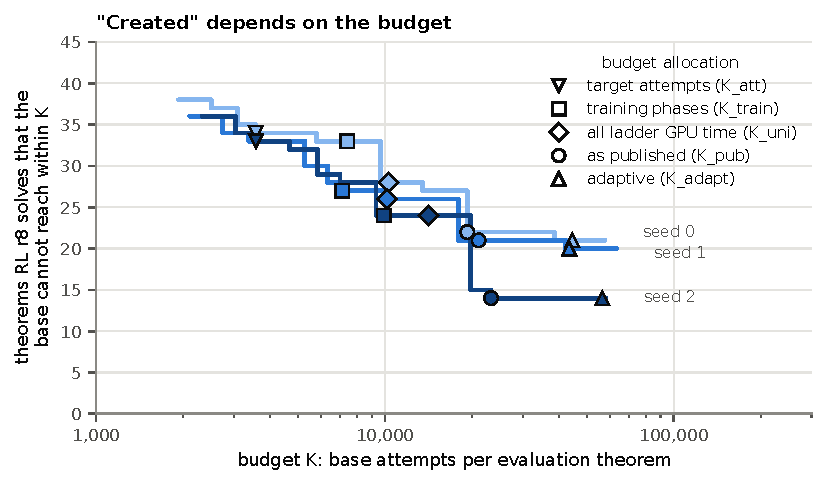
\includegraphics[width=0.66\linewidth]{figures/fig4_budget.pdf}
\caption{The compute-matched ``created'' set (RL r8 solves, the base cannot reach within $K$) against the base budget
$K$, for full-exposure seeds s0--s2. Markers are the five budget allocations of Table~\ref{tab:budgets}. Lines end
where the base data stop deciding membership.}
\label{fig:budget}
\end{figure}

\paragraph{$k$-to-solve intervals and the known-proof estimator.} Sampling gives $\hat p = c/n$ and a one-sided 95\%
Clopper--Pearson upper bound \ub{}. For rare events we add a lower estimate from likelihoods. The \emph{known-proof
estimate} $E(t)$ sums, over every Lean-accepted proof of $t$ that any model found, the base's teacher-forced probability
of that proof at $T=0.8$. The sum also runs over the environment's 33 naming offsets. The interval
$[1/\ub,\ 1/E]$ brackets the $k$-to-solve. $E$ is not a strict lower bound, because the sampler conditions on its own
names and unseen proofs are missing, so we calibrated it against large-$k$ sampling (Fig.~\ref{fig:estimator}). On
calibration theorems with 3--100 successes in 512, it recovers a median 0.98/0.94/0.93 of the measured $p$. Across 196
(seed, theorem) pairs with large-$k$ sampling, the median of $E/\hat p$ is 0.937 for $\hat p \geq 10^{-3}$ (106 pairs),
0.883 for $10^{-4}$--$10^{-3}$ (52), and 0.454 for $10^{-5}$--$10^{-4}$ (36). The estimate is usable in aggregate down
to about $10^{-4}$. Below that it runs about two-fold low, so a ``within reach if $E \geq 2/K$'' rule loses power
exactly where RL's budgets sit ($K \approx 10^4$). Sampling verdicts stay primary.

\paragraph{Certificates.} A theorem is \emph{certified out of reach at $K$} if $\ub < 0.05/K$. With zero successes
this needs about $60K$ attempts. We sampled the base 1.1--1.5 million times on 9 (theorem, seed) pairs from the
compute-matched sets: 7 of 9 certify at $\Kpub$. A pair \emph{survives every RL-free control} if it also has no success
from the replay-only control, from the compute-matched pretraining continuation, or from any other seed's base. Four
pairs on three theorems survive at $\Kpub$. Only one of the three theorems, a Peirce instance, is classical-only. Their
known proofs bound the base's $k$-to-solve from above at $10^{10}$--$10^{13}$. That is an extrapolation far outside
the estimator's calibrated range; sampling shows only $>4\times 10^5$.

\paragraph{RL-free controls.} Two controls receive RL's training without RL's proofs. The \emph{replay-only} control
fine-tunes pend for the same eight rounds on pretraining replay alone. It solves 239/244/249 of the 322, against pend's
232/236/234 and r8's 286/286/293. The \emph{continuation} control trains pend further on \KT{} for about 75--78\% of the
ladder's GPU time (same-class seconds). It solves 220/215/219: it gains 12--19 theorems and loses 30--42. At matched
gains in IRT ability, EI flags no more items as differentially improved than replay-only training. The weight update
of eight RL rounds is about as large as replay-only's (relative norm 0.28 vs 0.30, one seed). Twelve operational
definitions of ``created'' agree poorly: the mean pairwise Jaccard similarity of their sets is 0.29 at r8 and 0.34
at r16. Different seeds' RL ``creates'' different theorems.

\paragraph{Exact likelihoods along RL.} For theorems that RL newly solves, the worst step of r8's eventual proof rises
under teacher forcing (at $T=1$) from about $-6.2$ nats at pend to about $-1.3$ at r8, mostly by round 4. RL also lifts the
pretraining reference proofs of these theorems, about three times less. For theorems that neither pend nor r8 solves,
the reference proofs do not improve under RL. The likelihood view agrees with the budget view. RL concentrates
probability on proofs whose hardest step the base already rated within a few nats.

\paragraph{From measurement to intervention.} Every criterion above compares a model with its own base. The base
always \emph{could} have written the proof with some small probability, so each criterion only bounds that probability
from above at some budget. The knockout below changes the base itself.

\paragraph{The knockout decision rule (pre-registered).} A family is \emph{acquired} (at the bar) by a model if the
model solves at least 50\% of the family's strict held-out members in a plain read of 256 attempts. Per family, the
verdicts were fixed before the ladders ran:
\begin{itemize}
\item \emph{created}: at least 2 of 6 knockout seeds acquire the family at r16, and the knockout base is certified out
of reach on it;
\item \emph{needs exposure}: at most one knockout seed acquires it, and the full arm acquires it on more seeds
(one-sided Boschloo test, $p \leq 0.05$);
\item \emph{neither}: no seed acquires it;
\item \emph{undetermined}: any other outcome.
\end{itemize}
The primary test compares, per seed, the indicator ``at least one family at the bar at r16'' between the full and
knockout arms. With six seeds per arm, the test rejects at full/knockout acquisitions of $(3,0)$, $(5,1)$ or $(6,2)$.
An outcome of 0/6 knockout seeds bounds the per-seed creation rate below 0.39 (one-sided 95\%).

\section{Related work}\label{sec:related}\emph{[Pending.]}

\section{Discussion}
\label{sec:discussion}

\paragraph{What the knockout shows.} Without \sig{} in pretraining or replay, 16 rounds of this EI acquired no classical
family on any of six seeds. With it, full-exposure seeds gained 8--69 strict held-out theorems during the RL phase, and a
1\% dose was enough on three seeds. The pre-registered verdict, \textsc{needs exposure}, holds for converse
contraposition, the family the full bases mostly had before RL; for the others it is undetermined at six seeds. Beyond
the waiting-time null (post hoc), the knockout ladders raised their own rate of the free positive reductio: three reached
a strict training theorem sooner than their base rates predict. They did not raise it to a family.

\paragraph{Four readings of the null.}
\begin{enumerate}
\item \emph{\sig{} is out of the policy's reach.} This is false for five of six bases, which proved strict theorems with
\sig{} at large $k$, and for four of six under guided decoding at $k = 256$. Seed 0's base is certified out of reach only
for plain sampling, at one budget and with an 8\% margin; its guided evaluation proved a strict theorem.
\item \emph{EI samples too little.} At 32 attempts per theorem, EI's per-round budget on the strict theorems is about
4,000 attempts, against base rates near $10^{-6}$. That explains why most ladders saw nothing for many rounds. It does
not explain everything: three ladders reached strict theorems sooner than this null predicts ($p = 0.006$--$0.019$).
\item \emph{EI amplifies rare finds too slowly, or too narrowly.} Seed 5 wrote a free positive reductio in round 2 and did
not spread it in 14 more rounds. Seed 1 multiplied its free positive reductio more than tenfold in eight extra rounds and still
proved the same five held-out theorems. In EI a single new proof enters a fine-tuning mix of about 70,000 RL records (up
to four proofs for each of 4,495 theorems, each repeated four times) plus 20,000 replay records.
\item \emph{The knockout made the bases worse learners in general.} The general costs are a few theorems out of
hundreds, and the knockout's gains elsewhere are not clearly smaller (partly catch-up). The dose arm restores
acquisition while moving the constituents by about one point. This reading is not excluded, but it is not needed.
\end{enumerate}

\paragraph{Positive-only or signed updates?} Whether another RL algorithm would do better from the knockout bases is the
main open question. EI updates only on successes. GRPO also pushes down failures and gives a lone success in a group of
32 an advantage of $\sqrt{31} \approx 5.6$ standard deviations. That helps only after a first success: when all 32
attempts fail, the group baseline gives no gradient, so on the strict theorems GRPO at $k=32$ faces the same waiting time
as EI. The evidence cuts both ways.
\begin{itemize}
\item \textbf{Against EI-specificity.} In this organism, from the same full-exposure bases at equal sampled attempts,
GRPO did not prove more theorems than EI. Default and unlikeliness-weighted GRPO proved significantly fewer of the 322
(theorems solved only by GRPO vs only by EI: 15 vs 38, sign test $p = 0.0022$; 15 vs 44, $p = 0.0002$). A pass@4
advantage was level (33 vs 20, $p = 0.098$), ahead on the hardest theorems mostly through one seed. Interplay's 0\%
exposure null used GRPO \citep{zhang2025interplay}. A strategy removed at fine-tuning did not re-emerge under GRPO
\citep{krishnamurthy2026select}. In LLM reasoning EI matched or beat PPO \citep{havrilla2024teaching}.
\item \textbf{For EI-specificity.} Rejection-sampling fine-tuning plateaued where GRPO built new shortcuts
\citep{abdulsalam2026rewrite}, iterated RFT failed where RL composed functions \citep{yuan2025fgx}, and GRPO produced a
pattern family absent from its RL data \citep{park2025countdown}. Training on negative samples preserves breadth that
positive-only training loses \citep{zhu2025nsr}. In our earlier 3.2M organism, GRPO acquired a depth-3 nesting habit from
zero-rate bases where EI mostly did not (below).
\end{itemize}
GRPO has not been run on the reductio in any of our organisms. A GRPO arm from the six knockout bases, with per-seed
predictions written down first, is the decisive experiment. By sampling alone, only the seeds with a strict success
inside 16 rounds (1, 2, 5) could be rescued, so any further rescue would have to come from drift.

\paragraph{Earlier organisms.} The project studied related patterns in smaller organisms: 3.2M--85M-parameter models
that write whole proofs, pretrained on proofs of at most six lines (their RL proofs ran to seven or eight). They were
judged by an older in-house checker, with Lean confirmation where stated. Their criterion for \emph{igniting} a pattern
was at least 2\% of the targets that need it, much weaker than our family bar.
\begin{itemize}
\item \textbf{Reductio, required pools.} Four of eleven reductio-free bases emitted the strict reductio before RL
($8\times10^{-6}$--$2.3\times10^{-4}$ per sample), and exactly those four ignited under EI. First proofs arrived about
when $1/(rkN)$ predicts (rounds 1, 2, 6 and 6, against 0.2, 1.7, 2.6 and 6.2). The other seven stayed at 0 of 606.
In those pools every target needed the pattern, so a zero-rate base gave EI no training step at all. At 3.2M, 25M and
85M parameters the rates did not rise with size. A rare 85M base that read 0 of 300 after eight rounds produced its
first proof in round 13 when continued. Igniting arms saturated the seven-line targets and went no further, an analogue
of knockout seed 1's narrow spread.
\item \textbf{Injected data.} One fine-tuning step on a sibling's found proofs ignited all 11 dead arms. A single injected
proof ignited the reductio on two dead seeds, reaching 6 and 17 targets in the next round. Four unrelated generator
instances, and even four invalid pattern strings, ignited some arms. In the present organism, 16 demonstrations taught
excluded middle (35--37 of 39 members) to a base pretrained with no \texttt{DN}.
\item \textbf{Mixed pools.} Where EI could train on other proofs, it ignited a depth-3 nesting habit from zero on three
of five bases, decided during training rather than by sampling luck. GRPO ignited it on every surviving arm from two
zero-rate bases (12 of 12), where paired EI did so in 1 of 3. That habit was not needed for the targets, the zero rates
were measured with the older checker, and the checkpoints are lost.
\end{itemize}
The knockout fits these results only partly. As there, the base rate predicts which seeds move, and no ladder that
started at a pooled rate near $10^{-6}$ reached the family bar. Unlike the required pools, our mixed pool let the
knockout ladders' rate rise: by the earlier criterion, knockout seed 1 ignited at round 13, and three ladders reached
strict theorems sooner than their base rates predict. ``Needs exposure'' should therefore be read as ``needs exposure,
demonstrations, or perhaps a different update, for this EI to acquire the family within 16 rounds''.

\paragraph{An amplification threshold?} One might expect EI to amplify a composition once some training theorems' rates
are high enough for 32 attempts per round to hit them within a few rounds. Our data are mixed. Knockout seed 1 amplified
members its base proved at about $10^{-4}$, but its largest gain was on a member with no base success. Knockout seed 4's
base proved three members at $1.2$--$4.9\times10^{-4}$, and its ladder amplified none. Two doses cannot tell a threshold
from a graded response. The median likelihood of known proofs also misses it: the nearest dose and knockout bases are
within 0.7 nats, yet their outcomes differ by 28--56 theorems. The 0.1\% dose, and per-theorem rates on training
theorems at several checkpoints, would test it.

\paragraph{What transfers to larger models.} The protocol transfers: budgets matched to RL's compute and reported as
curves, RL-free controls, certificates. So does the waiting-time logic. A first success is expected after about
$1/(rkN)$ rounds, so with $10^4$--$10^5$ prompts and $k$ of 8--64, LLM RL can find far rarer compositions than our 123
strict theorems allow, if a comparable share of prompts needs them. The numbers do not transfer. Two practical points
follow, with that caveat.
\begin{itemize}
\item \textbf{Evaluation.} Absence at modest $k$ under plain sampling is not absence. Our knockout bases fail at $k=256$,
yet a million plain attempts or a guided evaluation at $k=256$ reveals the composition.
\item \textbf{Data filtering.} Removing a composition from pretraining kept this EI from acquiring it for 16 rounds, but
1\% of records restored it. We did not test the leakage levels a real filter leaves. In the same organism, 16
demonstrations taught a no-\texttt{DN} base excluded middle, so fine-tuning on demonstrations would likely defeat such a
filter.
\end{itemize}

\paragraph{An evidence hierarchy for ``RL created it''.} In increasing strength:
\begin{enumerate}
\item success at equal $k$;
\item a compute-matched base budget, reported as a curve over defensible allocations;
\item RL-free controls with matched training;
\item a certificate against the base at that budget;
\item an intervention on what the base saw.
\end{enumerate}
For our full-exposure seeds the claim shrinks at each step (Table~\ref{tab:budgets}). With the intervention, exposure was
followed by acquisition within 16 rounds, and its absence by none, for one composition and one algorithm. Steps 2 and 3
cost about as much as the RL run they audit, so they are affordable wherever that run was; they are rarely reported.

\section{Limitations}
\label{sec:limits}

\begin{itemize}
\item \textbf{Scale and domain.} One architecture with 9.56M parameters, propositional logic over at most four atoms,
and pretraining proofs of at most 12 lines. Nothing here is measured on a large language model or on first-order
logic. The organism was chosen because it allows interventions that large models do not. The price is that results
about it are results about it.
\item \textbf{One RL algorithm, 16 rounds.} T1 expert iteration with $k=32$ at $T=0.8$ is rejection-sampling
fine-tuning. GRPO-style updates, more exploration (higher temperature, larger $k$ on failed targets) or longer ladders
could behave differently. An earlier comparison from the same checkpoints found GRPO with a pass@4 advantage ahead of EI
on the hardest theorems, though mostly through one seed. ``Needs exposure'' is a statement about 16 rounds of this EI,
and one knockout seed was still changing at round 24.
\item \textbf{Seeds and power.} Six seeds per arm power the primary indicator but not most per-family tests. Three
families are 3 vs 0 (Holm 0.17), and excluded middle, acquired by one full seed, is untestable at these counts. A 0/6
outcome bounds the per-seed rate of creation below 0.39 only; creation in one seed out of ten would likely be missed.
The dose arm has three seeds.
\item \textbf{Near-saturated training targets.} By round 8 the full ladders solve 97--98\% of the 4,495 training
theorems. The classical families are a small part of the training signal, and the classical held-out members are hard.
A pool richer in classical targets might change the dynamics.
\item \textbf{The knockout is not surgical.} Besides \sig{}, it lowers the share of \texttt{DN} and $\neg$-introduction
records and the share of classical-only theorems. The knockout bases are 6.88 points worse at greedy held-out decoding
(all of it on theorems that need \sig) and solve fewer intuitionistic textbook72 theorems at pend ($-4.0$ of 53, three
full seeds). The textbook72 gap persists at r16.
\item \textbf{``Absent'' is not established.} Only 2 of 6 knockout bases are certified out of reach at RL's budget, and
no family is certified for any seed. The estimator that would quantify smaller rates runs two- to four-fold low below
$10^{-4}$ and was calibrated on full-exposure models. The likelihood scores use the full ladders' proofs and one naming
offset.
\item \textbf{Sharpening.} The power-sampling null holds for one Metropolis--Hastings sampler that fails its own
positive control. It says nothing about $p^\alpha$ itself.
\item \textbf{Cut-offs and settings.} Many plain reads cut off more than 0.1\% of attempts in some stratum (up to 8.8\%
of strict-member attempts on one dose seed). We re-read the strict members with doubled caps (\S\ref{sec:checks}). The
old and new full seeds differ in GPU class (RTX A6000 vs A40) and sampling batch for rounds 1--8, and are pooled. The
budget conversions rest on one measured class ratio.
\item \textbf{Measurement results are on three seeds.} \S\ref{sec:measure} uses the three earlier full-exposure seeds.
Its test-time-compute comparisons with guided reads are not compute-matched.
\end{itemize}

\section{Reproducibility}
\label{sec:repro}

\paragraph{Code, data and models.} All code is in the fork \texttt{dan-pandori/nd-takehome}. The experiments are on
branch \texttt{dan\_create-or-elicit} (commit \texttt{8e195390}, with the review): scripts \texttt{coe/} and
\texttt{pod/coe/}, the reviewer's independent recount code \texttt{review\_coe/}, the pre-registration, the per-round
statistics, the budget and estimator outputs, and the claims ledger. This paper is on \texttt{dan\_create-or-elicit-paper}.
Its figures and statistics are regenerated by \texttt{paper/scripts/} from those files, and every number in the text
has a row in \texttt{paper/LEDGER.md} pointing to its reviewed source. The pretraining sets, all 200 ladder
checkpoints, the read rows, the large-$k$ samples and the Lean-gate dumps are in the public bucket
\texttt{hf://buckets/dan-pandori/nd-rl/create-or-elicit/}. The decompressed md5 sums of the pretraining sets are
\KT{} \texttt{800b5486}, \KTko{} \texttt{466fc214} and \KTdose{} \texttt{19cd2263}.

\paragraph{Pre-registration and review.} The experiment's pre-registration was committed before the first GPU pod was
created. Six dated addenda each precede the work they govern, with one disclosed exception. Addendum 2 replaced the
held-out sets with the strict sets after the first round of the first knockout ladder. The reviewer's recount shows the
original sets give the same primary result. An independent reviewer re-derived every count in \S\ref{sec:results}
blind to the write-up, from the raw files and with separate code, and re-checked the proofs in Lean. The reviewer
corrected three Boschloo $p$-values computed on a transposed table (no verdict changed) and asked for ten rewordings.
This paper uses the corrected values and the reviewed wording. This writing run was pre-registered as well
(\texttt{preregistration/create-or-elicit-paper.md}), including the checks of Appendix~\ref{sec:checks}.

\paragraph{Compute.} Table~\ref{tab:compute} gives the compute per arm. Every 16-round ladder made 2,301,440 attempts
on training theorems and 9,600 fine-tuning steps. The knockout and dose ladders' compute is within 0.95--1.03 times the
full ladders' on every quantity. The experiments used 16 pods, 15 NVIDIA A40 (\$0.59/h) and one RTX A6000: 309.34
pod-hours and \$182.50 in total. The earlier runs whose results \S\ref{sec:measure} and \S\ref{sec:ttc} quote record
their compute in their own reports (Appendix~\ref{app:provenance}).

\begin{table}[h]
\centering\small
\caption{Compute per new 16-round ladder, mean over seeds (A40; results-registry rows, recounted by the reviewer).
Pretraining took a further $\approx$1,280 GPU-seconds, $\approx$24,000 steps and $\approx 4.4\times10^8$ tokens per
seed.}
\label{tab:compute}
\begin{tabular}{lrrr}
\toprule
quantity & \Kko{} & \Kfull{} (s3--s5) & \Kdose{} \\
\midrule
sampling GPU-s & 32,441 & 34,005 & 34,492 \\
evaluation GPU-s & 7,886 & 8,046 & 7,970 \\
fine-tuning GPU-s & 13,747 & 13,753 & 13,898 \\
total GPU-s & 54,105 & 55,841 & 56,390 \\
generated tokens & $6.69\times10^8$ & $6.73\times10^8$ & $6.76\times10^8$ \\
Lean checks & $2.15\times10^6$ & $2.21\times10^6$ & $2.18\times10^6$ \\
\bottomrule
\end{tabular}
\end{table}


\section*{Acknowledgements}
Left for Dan.

\bibliographystyle{plainnat}
\bibliography{refs}

\appendix
\section{Glossary}
\label{app:glossary}
\begin{description}[leftmargin=1.2em,style=nextline]
\item[pend, r$N$] the model at the end of pretraining; after $N$ rounds of expert iteration.
\item[plain read / guided read] $k=256$ independent attempts per theorem at $T=0.8$ / the same with logically rejected
steps redrawn (at most 10 per attempt). x0, x1: two sample seeds of a plain read.
\item[\sig, \sigp, lemma route] \texttt{DN} on a line built by $\neg$-introduction / \texttt{DN} on any derived line /
proving $\neg\neg G\to G$ inside an implication box and applying it.
\item[free positive reductio] \texttt{DN} on a derived line whose conclusion $G$ is not a negation and whose
$\neg\neg G$ is not a subformula of the theorem, by any route.
\item[strict member] a family member that is classical-only (no intuitionistic proof, by G4ip) and has no $\neg\neg$
subformula in its sequent.
\item[at the bar] a family with at least 50\% of its strict held-out members solved in a plain read.
\item[within reach at $K$] the base's empirical success rate $\hat p \geq 1/K$ over at least $K$ attempts.
\item[certified out of reach at $K$] one-sided 95\% Clopper--Pearson upper bound $< 0.05/K$.
\item[\dcov] theorems RL solves at $k=256$ minus theorems the base reaches within $K$.
\end{description}

\section{Construction of the knockout set}
\label{app:k12ko}
\KTko{} removes every \KT{} record whose written or pruned proof applies \texttt{DN} to a derived double negation
(16,961 records: 16,703 \sig{} and 258 whose \texttt{DN} cites an $\to$-elimination, $\lor$-elimination,
$\bot$-elimination, \texttt{DN} or $\land$-elimination line). It refills 16,961 records, drawn uniformly per length from
\KT{}'s own unused source pools: lengths up to 6 from the depth-3 generator pool and lengths 7--12 from the long-proof
pool. Every refill record passes every \KT{} filter (no box depth $\geq 3$; \texttt{DN} only on assumptions or
premises) and is \sigp-free and lemma-route-free. Under an order-sensitive and a premise-order-invariant renaming key,
the refill shares no class with \KT{} or with any of the 100 data and target files of the repository. One of \KT{}'s 11
exclusion pools was absent when the set was built and could not be checked. Every refill record's proof, translated to
Lean, is accepted (16,961/16,961). Unchanged proofs pass the same harness, and goal-negated proofs fail it. Removal and
refill leave the per-length counts identical. The dose set \KTdose{} swaps 1,550 refill records for removed \sig{}
records at \KT{}'s \sig{} length mix. A 0.1\% set is built but unused.

\section{When each ladder first trained on each family}
\label{app:shares}
First round in which at least half of a family's strict training targets had an accepted proof in the ladder (every
target receives 32 attempts per round; ``--'' = not within 16 rounds).
\begin{center}\small
\begin{tabular}{lcccccc}
\toprule
ladder & contrap.\ conv. & neg.\ cond. & Peirce & Peirce seq. & excl.\ middle & De Morgan \\
\midrule
\Kfull{} s0/s1/s2 & 1/2/1 & 4/13/3 & --/--/3 & --/--/5 & --/14/-- & never \\
\Kfull{} s3/s4/s5 & 2/1/1 & 2/--/-- & 8/--/-- & 3/--/16 & never & never \\
\Kko{} s0--s5 & never & never & never & never & never & never \\
\Kdose{} s0/s1/s2 & 2/1/3 & 3/7/7 & 12/--/-- & 7/--/-- & never & never \\
\bottomrule
\end{tabular}
\end{center}

\section{Budgets at r16 and the estimator}
\label{app:budgets}
At r16 the five allocations are $\Katt = 7{,}147$; $\Ktrain = 17{,}531/15{,}884/20{,}422$; $\Kuni =
24{,}619/22{,}827/29{,}510$; $\Kpub = 47{,}962/49{,}428/50{,}447$; $\Kadapt = 109{,}875/100{,}929/119{,}575$ base
attempts per theorem. Because $\Kadapt$ exceeds the 66,304 attempts most hard theorems received, the r16 sets at
$\Kadapt$ are mostly undetermined. Figure~\ref{fig:estimator} shows the known-proof estimator's calibration.

\begin{figure}[h]
\centering
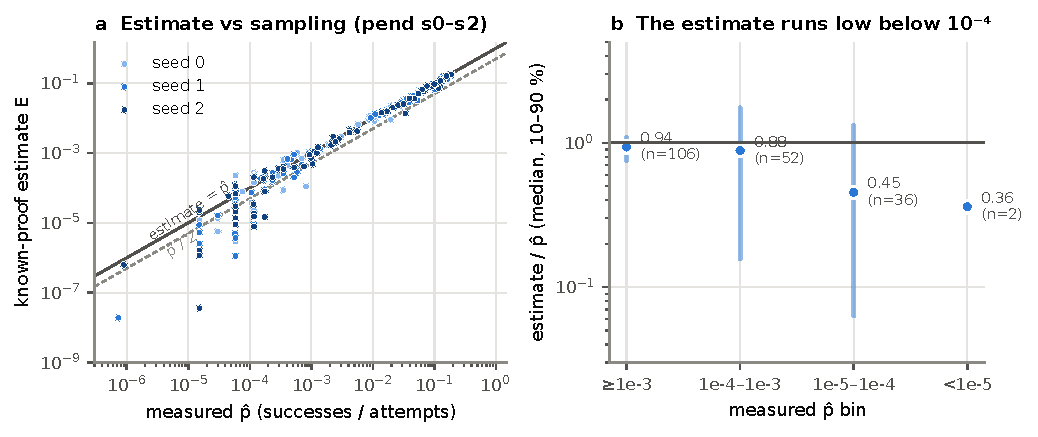
\includegraphics[width=0.92\linewidth]{figures/fig5_estimator.pdf}
\caption{Known-proof estimator, full-exposure bases s0--s2. (a) Estimate against measured $\hat p$ for (seed, theorem)
pairs with at least one success in large-$k$ sampling. (b) Median and 10--90\% range of $E/\hat p$ by $\hat p$ bin.}
\label{fig:estimator}
\end{figure}

\section{Power sampling}
\label{app:power}
The sampler targets $p^\alpha$ over whole proofs by Metropolis--Hastings with suffix resampling
(\texttt{coe/power\_sample.py}): 32 chains per theorem, blocks of 4 proof steps, 8 MH steps per block (32 in the
convergence check), $\alpha \in \{4, 2\}$ (and 1.5 in the control). Acceptance rates were 0.55--0.74. On a development
pilot the per-chain success was 0.752 at 8 MH steps per block and 0.760 at 32. The plain comparators received exactly
the decoded tokens of the power runs. They store no proof text, so their 1--2 solves could not be re-checked in Lean.

\section{Pre-registered expectations against outcomes}
\label{app:expectations}
The experiment's pre-registration stated numeric expectations. As tallied by the reviewer, they \emph{hit} on:
\begin{itemize}
\item the shape of \KTko{};
\item the general-ability gap on held-out greedy decoding and on non-\sig{} theorems;
\item 0/123 strict targets in round 1 and 0/106 held-out members at pend on all knockout seeds;
\item knockout median log-probabilities at or below $-15$ nats;
\item converse contraposition acquired on 3/3 new full seeds;
\item at least one family on 6/6 full and 0/6 knockout seeds;
\item the primary $p$ and the arm medians;
\item recovery of non-classical holdout250 by r16;
\item $\dcov > 0$;
\item the power-sampling nulls;
\item the dose arm's round-1 \sig{} proofs and family acquisition;
\item knockout seed 1's extension.
\end{itemize}
They \emph{missed} on:
\begin{itemize}
\item the classical-only share falling by $\geq 70\%$ (observed 67.6\%);
\item textbook72 within $\pm4$ (observed $-6.5$);
\item certificates on $\geq 5/6$ knockout bases (observed 2/6);
\item negated conditional on $\geq 2/3$ new full seeds (observed 1/3);
\item the first \sigp{} proof after round 4 (it appeared in round 1, on theorems supplying $\neg\neg G$);
\item $\dcov$ within $+8$ to $+35$ (two seeds at $+36$ and $+37$);
\item 0/106 for every sampler on the knockout bases (plain sampling at $T=1$ solved one);
\item 3--15 strict targets in the dose arm's round 1 (observed 2/17/2);
\item a seeded-round gain on $\geq 3$ seeds (observed 1/5).
\end{itemize}

\section{Corrections applied}
\label{app:corrections}
The experiment's own scripts passed two-by-two tables to \texttt{scipy.stats.boschloo\_exact} with the groups as rows.
That function treats columns as groups. With the arms as columns, the RL-only test is $p = 0.0032$ (reported 0.0020),
the excluded-middle test $0.39$ (0.30) and the three-versus-none family tests $0.034$ (0.035). The primary
$p = 0.00024$ and the dose test $p = 0.0033$ are unchanged. \texttt{paper/scripts/stats\_extra.py} recomputes all
five. The reviewer's ten rewordings are applied throughout. The most important ones: ``need'' becomes ``not acquired by
this EI within 16 rounds'', ``reach'' is used only in its technical sense, and the sharpening null is stated for one
sampler.

\section{This paper's checks}
\label{sec:checks}
\emph{[Pending: the pre-registered checks C1--C3 are running; results will be filled in here.]}


\section{Provenance of earlier results}
\label{app:provenance}
Run names refer to reviewed reports in the fork \texttt{dan-pandori/nd-takehome} (branch \texttt{dan\_<run>}, file
\texttt{review\_<run>.md}) and to their summaries in \texttt{nd-rl/experiment-summaries}.
\begin{itemize}
\item \run{create-or-elicit}: the knockout, dose and full s3--s5 ladders; Phase 0 (budgets, estimator) and Phase 2
(power sampling). Review commits \texttt{dd8ee82e} (blind recount), \texttt{8e195390} (verdict).
\item \run{capability-defs}: the measurement framework on full seeds s0--s2 (budgets, certificates, controls,
definitions, guided reads). Review \texttt{da11be78}.
\item \run{trajectory}, \run{rl-continue}: full seeds s0--s2, rounds 1--8 and 9--16; exact likelihoods along RL.
\item \run{rl-from-ckpt}: the replay-only control.
\item \run{guided-tts}: guided redraws at matched tokens; the step checker.
\item \run{mcts-a}: PUCT search with a learned value (review \texttt{5e70afbd}).
\item \run{grpo-best}: GRPO variants from the same checkpoints.
\item \run{support-curves}, \run{support-state}, \run{claim-audit}: the 3.2M organism and the interface confound.
\end{itemize}
The claims ledger (\texttt{claims\_ledger.md}, rows L1--L101) maps every inherited number to its reviewed source.


\end{document}
